\documentclass[a4paper,12pt]{article}
\usepackage{float} % en el preámbulo

% Paquetes básicos
\usepackage[utf8]{inputenc}
\usepackage[spanish]{babel}
\usepackage{amsmath, amssymb}
\usepackage{graphicx}
\usepackage{geometry}
\usepackage{hyperref}
\geometry{margin=2.5cm}

% Datos del informe
\title{Inferencia Y Estimación}
\title{Título del Informe}
\author{Catalina Hirsch - 36557 \\ Clara Zavaroni Benoit - 36772 \\ Maylen Antonella Villagran Cardozo - legajo \\ \\ Universidad de San Andrés}
\date{\today}

\begin{document}

\maketitle

\begin{abstract}
La realización de este trabajo práctico tiene como objetivo aplicar el método de 
PCA en la compresión de imágenes. De esta manera, se busca reducir su espacio de almacenamiento,
minimizando la pérdida de información, conservando los datos que contengan la mayor parte de la información.
Luego, se descomprime la imagen y se compara con la original para evaluar la calidad de la compresión. 
Para ello, se evalúa su desempeño basado en la cantidad de componentes principales utilizados.
Finalmente, pudimos observar que,....
\end{abstract}

\section{Ejercicio 1}
El propósito de este ejercicio consiste en analizar el comportamiento de los píxeles vecinos en las imágenes utilizadas.
En primer lugar, se cargan las imágenes y se convierten a escala de grises. Luego, se divide cada imagen en bloques de 2x1 píxeles
contiguos verticalmente. A continuación, se calcula la correlación entre los píxeles de cada bloque y se almacena en un vector.
Finalmente, se realiza un gráfico de dispersión de las correlaciones obtenidas para cada imagen.
Los resultados se presentan a continuación:
\\
Para la primer imagen podemos observar la correlación de los píxeles contiguos verticalmente:

\begin{figure}[H]
    \centering
    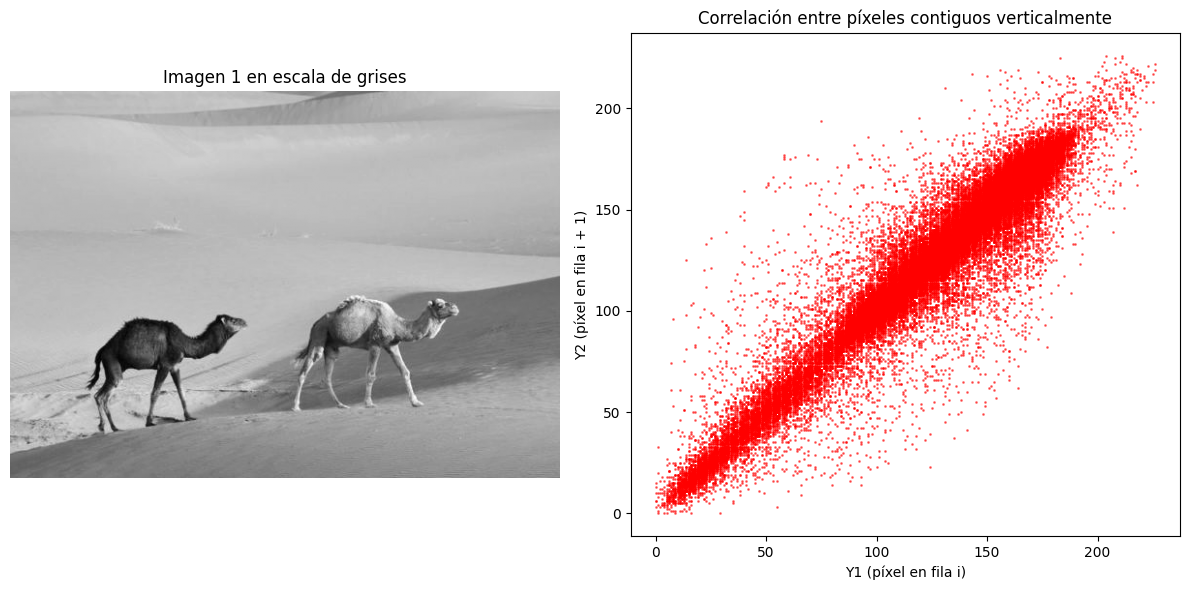
\includegraphics[width=1\textwidth]{Ejercicio1a.png}
    \caption{Imagen 1, gráfico de dispersión de la correlación de píxeles contiguos verticalmente}
    \label{fig:correlacion1}
\end{figure}

Analizando el comportamiento del gráfico, los puntos se alinean en torno a una recta creciente, lo cuál indica una fuerte correlación positiva entre los píxeles.
El resultado se debe a que, la imagen presenta suavidad, el color de los píxeles vecinos se asemeja.

Por otro lado, los resultados de la segunda imagen son los siguientes:

\begin{figure}[H]
    \centering
    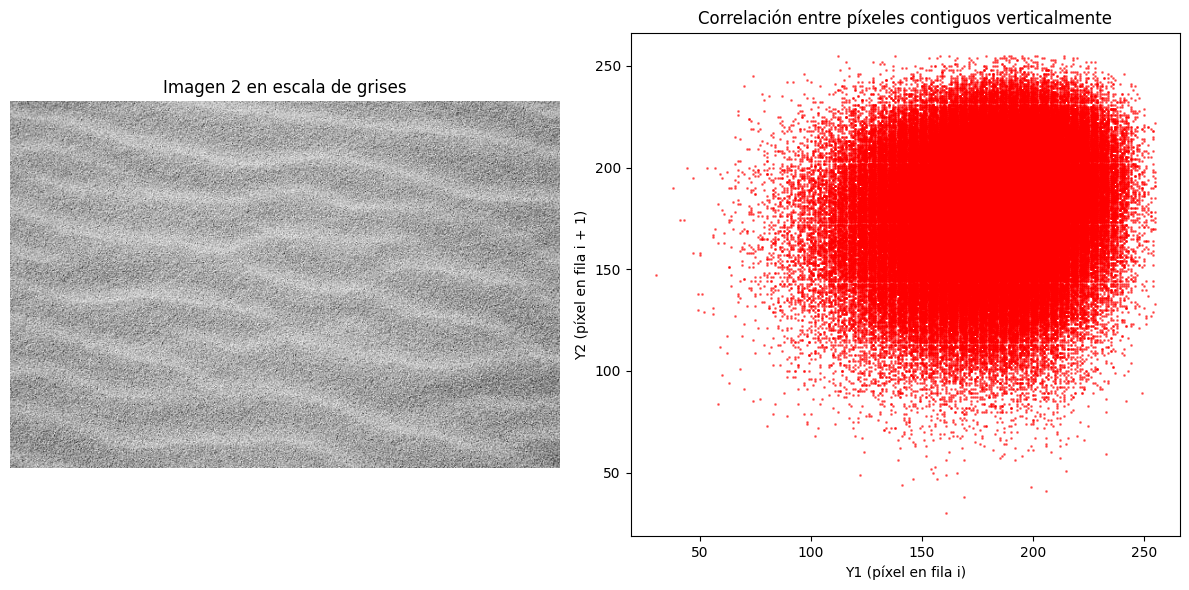
\includegraphics[width=1\textwidth]{Ejercicio1b.png}
    \caption{Imagen 2, gráfico de dispersión de la correlación de píxeles contiguos verticalmente}
    \label{fig:correlacion2}
\end{figure}

A diferencia del gráfico anterior, los puntos se encuentran más dispersos, implicando una correlación más baja que la imagen anterior.
Atribuímos la diferencia al ruido perteneciente a esta imagen, y a la falta de suavidad. Los colores entre los píxeles vecinos no están relacionados.
\\
Luego, se estiman los coeficientes de correlación de cada vector siguiendo el proceso:

\begin{enumerate}
    \item Se separa la imagen en bloques de 8 * 8
    \item Para cada bloque, se utiliza .flatten() para convertir en un vector 64 * 1
    \item Para el calculo de la correlación, se calcula el desvio estándar de cada par de vectores contiguos verticalmente. 
    Evitando la posible división por cero en el calculo.
    \item Se calcula la correlación entre vectores contiguos verticalmente.
\end{enumerate}

Los resultados son los presentados a continuación:
\begin{enumerate}
    \item Para la Imagen 1 se obtuvieron valores como: 
    $[-0.67, -0.69, -0.48, 0.19, \dots]$, 
    con una media de $\bar{\rho}_1 = 0.0993$. 

    \item Para la Imagen 2 los coeficientes fueron: 
    $[0.007, 0.276, -0.017, -0.052, \dots]$, 
    con una media de $\bar{\rho}_2 = 0.0022$.
\end{enumerate}

Los resultados de la primer imagen apoyan lo intuido anteriormente, al aproximarse al valor 1, indican una fuerte correlación entre los píxeles.
Con respecto a la segunda imagen, sus resultados también apoyan lo intuido, al acercase al valor 0, demuestra que los píxeles vecinos no están relacionados.

Por último, se pide una transformación que descorrelacione las variables.
Se utiliza la transformación de descorrelación de PCA:

\[
Y = P^T X
\]
De esta forma, \(Y\) es la proyección de \(X\) en el espacio de autovectores de \(C_X\).
\\
Nuevamente, se hace uso de un gráfico de dispersión por imagen, dando los siguientes resultados:

\begin{figure}[H]
    \centering
    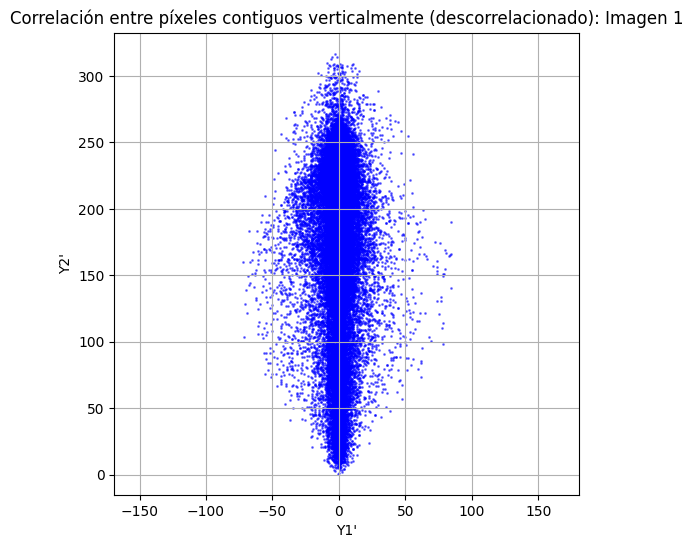
\includegraphics[width=0.7\textwidth]{Ejercicio1c.png}
    \caption{Imagen 1, gráfico de dispersión de la descorrelación de píxeles contiguos verticalmente}
    \label{fig:descorrelacion1}
\end{figure}

Podemos observar en la primer imagen, como los píxeles se encuentran concentrados en el eje vertical Y2, el proceso de descorrelación resulta exitoso.

\begin{figure}[H]
    \centering
    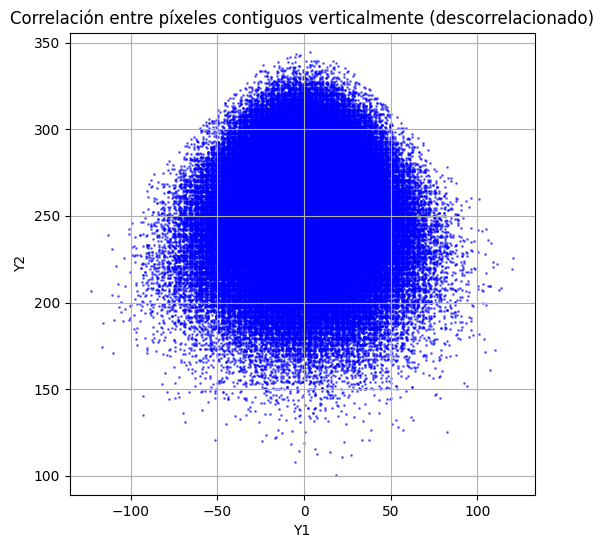
\includegraphics[width=0.7\textwidth]{Ejercicio1d.png}
    \caption{Imagen 2, gráfico de dispersión de la descorrelación de píxeles contiguos verticalmente}
    \label{fig:descorrelacion2}
\end{figure}

Por otro lado, en la segunda imagen, el gráfico se mantiene en forma de una nube, como en la Figura 2. Demostrando la falta de correlación inicial.

\section {Ejercicio 2}

\section {Ejercicio 3}

Luego de lo realizado en el Ejercicio 2, se realiza la reconstrucción de la imagen comprimida. Utilizando el proceso inverso del PCA de compresión, para descomprimir.
A través del Ejercicio 2, se obtienen los siguientes datos de la imagen:

Vectores \(y_i\) (\(Y\)), la matriz de autovectores (\(P\)) y la media \(\mu_X\) (\(\mu\))

Una vez obtenida la información indicada, se aplica la proyección inversa del PCA, para obtener los vectores \(x_i\) aproximados:

\[
X = Y P^T + \mu
\]
donde \(X\) es la matriz original, \(Y\) es la matriz proyectada, \(P\) son los autovectores y \(\mu\) es la media.
\\
Finalmente, se recorre una matriz vacía, del tamaño necesario de la imagen. Completando con los bloques de la imagen reconstruída.
De esta manera, obtenemos los siguientes resultados:

\begin{figure}[H]
    \centering
    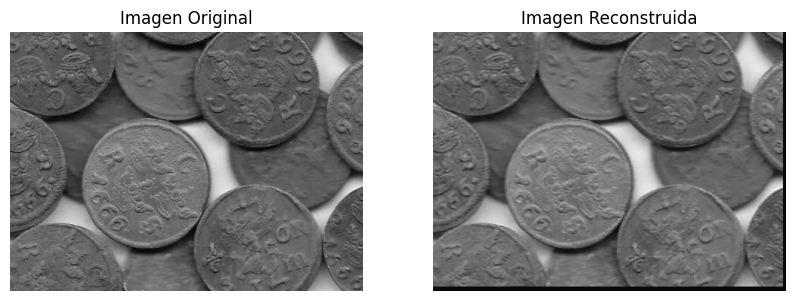
\includegraphics[width=1\textwidth]{Ejercicio3.png}
    \caption{Imagen reconstruida a través del proceso de PCA inverso.}
    \label{fig:ej3}
\end{figure}

Podemos notar el borde negro de la imagen reconstruida, lo cuál sucede al no poder completar bloques de exactamente 8 * 8 al comprimir la imagen.
Adicionalmente, podemos observar una diferencia entre las imágenes o pérdida de nitidez, atribuido a la reducción de la dimesionalidad y la eliminación de componentes de menor varianza.

\section{Ejercicio 4}
El objetivo de este ejercicio es evaluar el desempeño de la compresion de imagenes al variar el espacio ahorrado (S). 

\begin{equation}
S = \left( 1 - \frac{\text{cantidad de componentes principales } (k)}{\text{cantidad de componentes totales } (m)} \right) \times 100 \%
\end{equation}

En primer lugar, para cada porcentaje de espacio ahorrado comprimimos una imagen y la reconstruimos. Luego, para medir el rendimiento del procedimiento, calculamos el error cuadratico medio (MSE) entre la imagen original y la reconstruida. 
\begin{equation}
MSE = \frac{1}{N_w N_h} \sum_{i=1}^{N_w} \sum_{j=1}^{N_h} (p_{ij} - \hat{p}_{ij})^2
\end{equation}

*insertar grafico*
En el grafico, se observa que el error cuadratico medio aumenta a medida que lo hace el espacio ahorrado. Este resultado es coherente, ya que al descartar un mayor numero de componentes principales se pierde mas informacion de la imagen. 

Para ilustrarlo, incluimos algunas imagenes para diferentes porcentajes de espacio ahorrado. 
*instertar imagenes*.
Vemos que a medida que S aumenta, la imagen reconstruida pierde nitidez. La reduccion de componentes principales se ve en una disminucion de la calidad de la imagen. 


\section{Metodología}
Explique los métodos, materiales y procedimientos utilizados.

\section{Resultados}
Presente los resultados obtenidos, incluyendo tablas y figuras si es necesario.

\section{Discusión}
Analice e interprete los resultados, comparando con la literatura o expectativas.

\section{Conclusiones}
Resuma los hallazgos principales y posibles trabajos futuros.

\section*{Referencias}
\bibliographystyle{plain}
\bibliography{referencias}

\end{document}